\chapter{Hyperbolic Equations in Two Variables : Elliptic, Hyperbolic \&\ Parabolic Operators}

\chaptermark{Hyperbolic Equations in Two Variables...}

\setcounter{pageoriginal}{0}
Let\pageoriginale $\Omega$ be an open set in $\mathbb{R}^{2}$ and
$$
L=A\frac{\partial^{2}}{\partial x^{2}}+2B\frac{\partial^{2}}{\partial x\partial y}+C\frac{\partial^{2}}{\partial y^{2}}+D\frac{\partial}{\partial x}+E\frac{\partial}{\partial y}+G
$$
be a second order linear differential operator in $\Omega$ where $(A,B,\ldots,G)$ are smooth $(c^{\infty})$ functions in $\Omega$.

\begin{defi*}
Let $(x_{0},y_{0})\in \Omega$. We say that the operator $L$ is elliptic at $(x_{0},y_{0})$ if the characteristic form
$$
A(x_{0},y_{0})\xi^{2}_{1}+2B(x_{0},y_{0})\xi_{1}\xi_{2}+C(x_{0},y_{0})\xi^{2}_{2}
$$
is definite i.e. if $(B^{2}-AC)(x_{0},y_{0})<0$. $L$ is said to be hyperbolic at $(x_{0},y_{0})$ if the characteristic form is indefinite i.e. $(B^{2}-AC)(x_{0},y_{0})>0$.
\end{defi*}

$L$ is said to be elliptic (resp. hyperbolic) in $\Omega$ if it is elliptic (resp. hyperbolic) at all points of $\Omega$. We shall define (provisionally) $L$ to be parabolic if the characteristic quadratic form is of rank 1 at every point.

\section*{The Wave Operator in Two Dimensions:}

We consider the wave operator $\dfrac{\partial^{2}}{\partial t^{2}}-\dfrac{\partial^{2}}{\partial x^{2}}$. The characteristic form is $\xi^{2}_{2}-\xi^{2}_{1}$. So this is an hyperbolic operator.

Make the change of variables $\xi=x+t$, $\eta=x-t$. We then have
$$
\frac{\partial}{\partial x}=\frac{\partial}{\partial \xi}+\frac{\partial}{\partial \eta}\quad\text{and}\quad \frac{\partial}{\partial t}=\frac{\partial}{\partial \xi}-\frac{\partial}{\partial\eta}\quad\text{so that}
$$
the wave operator goes over into the operator $4\dfrac{\partial^{2}}{\partial \xi \partial \eta}$.

Let\pageoriginale us consider the operator $\dfrac{\partial^{2}}{\partial \xi \partial \eta}$. The characteristic form is $\xi_{1}\xi_{2}$. A curve $C$ defined by $\phi=0$ with $d\phi\neq 0$ on $C$ will be characteristic if $\dfrac{\partial \phi}{\partial \xi}\cdot \dfrac{\partial \phi}{\partial \eta}=0$. We see that the curves $\xi$ = constant and $\eta$ = const. are characteristic curves.

If we look at the Cauchy problem $\dfrac{\partial^{2}u}{\partial\xi\partial\eta}=0$ and
$$
u(\xi,0)=\phi_{0}(\xi), \ \dfrac{\partial u}{\partial ???}(\xi,0)=\phi_{1}(\xi)\quad\text{on}\quad \eta=0,
$$
we see from
$$
\dfrac{\partial^{2}u}{\partial \xi \partial \eta}=0, \ \dfrac{\partial}{\partial \xi}\left(\dfrac{\partial u}{\partial \eta}\right)=0
$$
that $\phi_{1}(\xi)$ is constant. The curve $\eta=0$ is characteristic and we see that the Cauchy data cannot be prescribed arbitrarily; some compatibility conditions have to be satisfied. Even if we take $\phi_{1}(\xi)$ to be a const. say $C$, the solution is not unique: take $u(\xi,\eta)=\phi_{0}(\xi)+f(\eta)$ where $t$ is any function with $f'(0)=C$ and $f(0)=0$.

From $\dfrac{\partial^{2}u}{\partial \xi\partial\eta}=0$ we have $\dfrac{\partial}{\partial\eta}\left(\dfrac{\partial u}{\partial\xi}\right)=0$ so that
$$
\frac{\partial u(\xi,\eta)}{\partial \xi}=f(\xi)
$$
so that $u(\xi,\eta)=\int f(\xi)d\xi+G(\eta)$, $G(\eta)$ being the constant of integration. Thus $u=F(\xi)+G(\eta)$; if $F(\xi)$ and $G(\xi)$ are smooth functions, it is clear that $F(\xi)+G(\eta)$ is a solution. Going back to the original variables, we see that
$$
u(x,t)=F(x+t)+G(x-t)
$$
is a solution of the wave operator.

We seek the solution of the Cauchy problem for the wave operator with initial data $u(x,0)=f(x)$; $\dfrac{\partial u}{\partial t}(x,0)=g(x)$, in the form $u=F(x+t)+G(x-t)$. We must have 
$$
u(x,0)=F(x)+G(x)=f(x)
$$\pageoriginale
and
$$
\frac{\partial u}{\partial t}(x,0)=F'(x)-G'(x)=g(x).
$$
Differentiating the first equation, we have $F'(x)+G'(x)=f'(x)$.

\smallskip

Thus $F'(x)=\dfrac{f'(x)+g(x)}{2}$  \ and \ $G'(x)=\dfrac{f'(x)-g(x)}{2}$ \ or
\begin{align*}
F(x) &= \dfrac{f(x)}{2}+\dfrac{1}{2}\int\limits^{x}_{0}g(\xi)d\xi+C_{1}\\[3pt]
G(x) &= \dfrac{f(x)}{2}-\dfrac{1}{2}\int\limits^{x}_{0}g(\xi)d\xi+C_{2}
\end{align*}

From $u(x,0)=f(x)$ we see that $C_{1}+C_{2}=0$. Hence
$$
u(x,t)=\dfrac{1}{2}\{f(x+t)+f(x-t)\}+\frac{1}{2}\int\limits^{x+t}_{x-t}g(\xi)d\xi.
$$

\begin{theorem*}
If $f$ is $C^{2}$ function and $g$ a $C^{1}$ function on $\mathbb{R}$, then the function $u(x,t)$ defined by
$$
u(x,t)=\dfrac{f(x+t)+f(x-t)}{2}+\dfrac{1}{2}\int\limits^{x+t}_{x-t}g(\xi)d\xi
$$
is a $C^{2}$ function in $t\geq 0$ and solves the Cauchy problem
$$
\begin{cases}
\dfrac{\partial^{2}u}{\partial t^{2}}-\dfrac{\partial^{2}u}{\partial x^{2}}=0\quad\text{in}\quad t\geq 0\\[5pt]
u(x,0)=f(x)\\[3pt]
\dfrac{\partial u}{\partial t}(x,0)=g(x).
\end{cases}
$$
\end{theorem*}

\begin{proof}
{\bf Exercise:}

The above solution of the Cauchy problem is called d'Alembert's solution.

Note the value of $u$ at $(x_{0},t_{0})$ depends only on the values of $f$ and $g$ on the closed interval $(x_{0}-t_{0}, x_{0}+t_{0})$ on the $x$-axis. These are the points\pageoriginale cut out on the axis by the characteristics $x-t=(x_{0}-t_{0})$ (= const.) and $x+t=(x_{0}+t_{0})$ passing through $(x_{0},t_{0})$. For this reason, the interval $(x_{0},-t_{0},x_{0}+t_{0})$ is called the interval or domain of dependence of the point $(x_{0},y_{0})$ (with respect to the wave operator).
\begin{figure}[H]
\centering
\includegraphics{chap1/1.eps}
\end{figure}

Conversely the initial values at a point $(\xi,0)$ on the $x$ - axis influence $u(x,t)$ only at points $(x,t)$ in the region bounded by the
\begin{figure}[H]
\centering
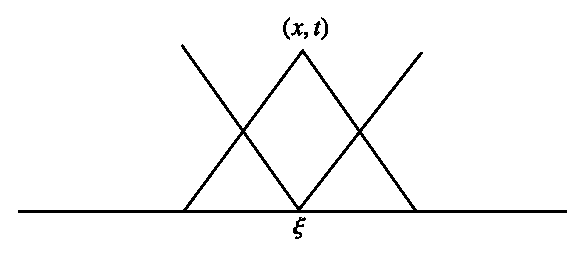
\includegraphics{chap1/2.eps}
\end{figure}
\noindent
characteristics $x+t=\xi$, $x-t=\xi$ i.e. in the region $\xi-t\leq x\leq \xi+t$. For this reason this region is called the domain of influence of the point $(\xi,\phi)$ on the $x$-axis.
\end{proof}

\begin{exer*}
Suppose that $f$ and $g$ have compact supports. Show that for each fixed $t$, the function $x\to u(x,t)$ has compact support.
\end{exer*}

Since any solution of $\dfrac{\partial^{2}u}{\partial t^{2}}-\dfrac{\partial^{2}u}{\partial x^{2}}=0$ is of the form $F(x+t)+G(x-t)$ the solution to the Cauchy problem is unique and is given by d'Alembert's formula.

\begin{exer*}
Let\pageoriginale $\{f_{n}\}$ (resp. $\{g_{n}\}$) be a sequence of $C^{2}$ (resp. $C^{1}$) functions which converges uniformly on compact subsets of $\mathbb{R}$ to a $C^{2}$ function $f$ (resp. $C^{1}$ function $g$). Show that the d'Alembert solution $u_{(f_{n},g_{n})}$ corresponding to the Cauchy data $(f_{n},g_{n})$ converges to the d'Alembert solution $u_{(f,g)}$ uniformly compact subsets of the upper half plane $t>0$.
\end{exer*}

Thus the Cauchy problem for the wave operator is well-posed.

\section*{Cauchy Problem for the Nonhomogeneous Wave Equation:}

We consider the Cauchy problem
\begin{gather*}
\frac{\partial^{2}u}{\partial t^{2}}-\frac{\partial^{2}u}{\partial x^{2}}=F(x,t)\quad\text{it}\quad t\geq 0;\quad u(0,x)=f(x),\\[4pt]
\frac{\partial u}{\partial t}(0,x)=g(x),
\end{gather*}
where $F$, $f$ and $g$ are given. We will derive an explicit formula for the solution by applying Green's formula.

Let $\Omega$ be a bounded domain with piecewise smooth boundary. Let $u$ be a real valued function on $\Omega$. We shall say that $u$ is of class $C^{k}$ in $\overline{\Omega}$ if $u$ is of class $C^{k}$ in $\Omega$ and if $u$ and all partial derivatives of order upto $k$ admit continuous extensions to $\overline{\Omega}$. We shall denote the extended functions also by the original symbol.

\begin{exer*}
Let $\Omega$ be the interior of the rectangle (OABC).
\begin{figure}[H]
\centering
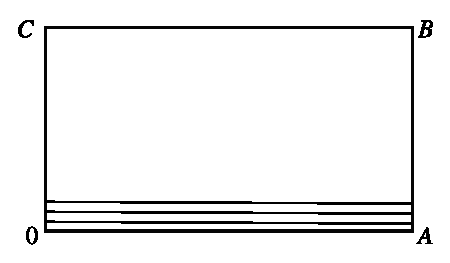
\includegraphics{chap1/3.eps}
\end{figure}
\noindent
where\pageoriginale $0A$ and $0B$ are the $x$ and $y$ axis. Let $f$ be a $C^{1}$ function on $\Omega$. Let $g(x)=f(x,0)$. Show that $g(x)$ is a $C^{1}$ function in the open interval $(0,A)$. Hint: (Consider a sequence of lines parallel to the $x$-axis and contained in the rectangle converging to $0A$).
\end{exer*}

We recall

\medskip
\noindent
{\bf Green's Formula:}~ Let $P$ and $Q$ be sufficiently smooth functions in $\overline{\Omega}$ where $\Omega$ is a bounded domain in $\mathbb{R}^{2}$ with a piecewise smooth boundary $\partial \Omega$. Then we have
$$
\iint_{\Omega}\left(\frac{\partial Q}{\partial x}-\frac{\partial p}{\partial y}\right)dx \ dy =\int\limits_{\partial \Omega}\ Pdx +Qdy.
$$
(The boundary is oriented ``anti-clockwise'')

\begin{coro*}
If $u$ is smooth, we have
$$
\iint\limits_{\Omega}\left(\frac{\partial^{2}u}{\partial t^{2}}-\frac{\partial^{2}u}{\partial x^{2}}\right)dx \ dt = \int\limits_{\partial\Omega}-\frac{\partial u}{\partial t}dx-\frac{\partial u}{\partial x}dt
$$

Apply this formula to the triangular region bounded by the characteristics $x-t=x_{0}-t_{0}$, $x+t=x_{0}+t_{0}$ and the $x$ - axis, where
\begin{figure}[H]
\centering
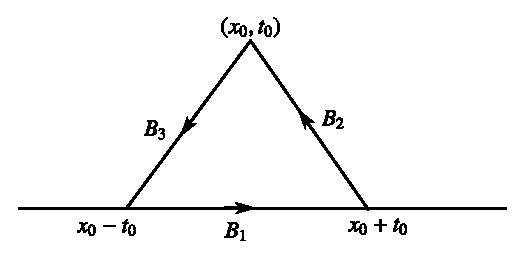
\includegraphics{chap1/4.eps}
\end{figure}
\noindent
$(x_{0},t_{0})$ is a point with $t_{0}>0$. If $u$ satisfies $\dfrac{\partial^{2}u}{\partial t^{2}}-\dfrac{\partial^{2}u}{\partial x^{2}}=F$, we have
$$
\int\limits_{B_{1}+B_{2}+B_{3}}-\frac{\partial u}{\partial t}dx-\dfrac{\partial u}{\partial x}dt=\int\limits_{\partial \Omega}-\frac{\partial u}{\partial t}dx-\dfrac{\partial u}{\partial x}dt=\int\limits_{\Delta} F\,dx\,dy
$$
where\pageoriginale $\Delta$ is in the interior of the triangle with vertices $(x_{0}-t_{0},0)$, $(x_{0}+t_{0},0)$, $(x_{0},t_{0})$ and $B_{1}$, $B_{2}$, $B_{2}$ are the sides of the triangle as indicated in the figure with their orientations.
\begin{enumerate}
\renewcommand{\labelenumi}{\rm(\theenumi)}
\item $\int\limits_{B_{1}}-\dfrac{\partial u}{\partial t}dx-\dfrac{\partial u}{\partial x}dt=-\int\limits^{x_{0}+t_{0}}_{x_{0}-t_{0}}\dfrac{\partial u}{\partial t}dx$

\item To evaluate the integral over $B_{2}$ consider the ``parametrisation'' $\phi(s)=(-s,s+x_{0}+t_{0})$ for $s$ in the closed interval $(-x_{0}-t_{0},-x_{0})$. We have $\phi(-x_{0}-t_{0})=(x_{0}+t_{0},0)$ and $\phi(x_{0})=(x_{0},t_{0})$. Since $dx=-dx$, $dt=ds$, and $\dfrac{d}{ds}=-\dfrac{\partial}{\partial x}+\dfrac{\partial}{\partial t}$
\begin{align*}
\int\limits_{B_{2}} \left(-\dfrac{\partial u}{\partial t}dx-\dfrac{\partial u}{\partial x}dt\right) &= \int\limits^{-x_{0}}_{-x_{0}-t_{0}}\left(\frac{\partial u}{\partial t}-\frac{\partial u}{\partial x}\right)ds\\[4pt]
&= \int\limits^{-x_{0}}_{-x_{0}-t_{0}}\left(\frac{du}{ds}\right)ds\\[4pt]
&= u(x_{0},t_{0}), u(x_{0}+t_{0},0)
\end{align*}

\item Consider the parametrisation of $B_{3}$ given by
$$
\psi(s)=(-s,-s-(x_{0}-t_{0}))
$$
for $s$ in the interval
$$
(-x_{0},-x_{0}+t_{0})\quad\text{with}\quad \psi(-x_{0})=(x_{0},t_{0}), \ \psi(-x_{0}+t_{0})=(x_{0}-t_{0},0).
$$

We have, as before
\begin{align*}
\int\limits_{B_{3}}\left(-\frac{\partial u}{\partial t}dx-\frac{\partial u}{\partial x}dt\right) &= \int\limits^{-x_{0}+t_{0}}_{-x_{0}}\left(\frac{\partial u}{\partial t}+\frac{\partial u}{\partial x}\right)ds\\[4pt]
&= -\int\limits^{-x_{0}+t_{0}}_{-x_{0}}\left(\frac{du}{ds}\right)ds\\[4pt]
&= u(x_{0},t_{0})-u(x_{0}-t_{0},0)
\end{align*}
\end{enumerate}

From\pageoriginale
$$
\int\limits_{B_{1}+B_{2}+B_{3}}=\int\limits_{\Delta}F \ dx \ dy,
$$
we get, from (1), (2) and (3) that
$$
u(x_{0},t_{0})=\frac{1}{2}\left\{u(x_{0}-t_{0},0)+u(x_{0}+t_{0},0)+\int\limits^{x_{0}+t_{0}}_{x_{0}-t_{0}}\left.\frac{\partial u}{\partial t}\right|_{t=0}dx+\int\limits_{\Delta} F \ dx \ dy\right\}
$$
\end{coro*}

\section*{Formula for the Solution of the Cauchy Problem:}\pageoriginale

What we have done above can be generalised a bit.
\begin{figure}[H]
\centering
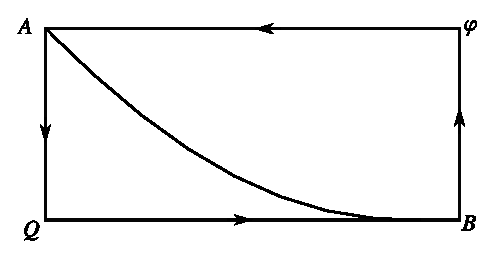
\includegraphics{chap1/5.eps}
\end{figure}

Let $S$ be a non-characteristic curve for the equation $\dfrac{\partial^{2}}{\partial x \partial y}$ i.e., $S$ is nowhere tangential to the lines $x$ = const. or $y$ = const. (More precisely the curve is given by $y=\sigma(x)$ with $\sigma'(x)<0$). Let $u$ be a solution of $\dfrac{\partial^{2}u}{\partial x\partial y}=F$ in the closed region $\overline{\Omega}$ bounded by $ABP$. We have by Green's formula
$$
\int\limits_{\Omega}\frac{\partial^{2}u}{\partial x\partial y}dx \ dy =\int\limits_{\partial\Omega}\frac{\partial u}{\partial y}dy=-\int\limits_{\partial \Omega}\frac{\partial u}{\partial x}dx
$$
Write these in the symmetrical form:
$$
\int\limits_{\Omega}\frac{\partial^{2}u}{\partial x\partial y}dx \ dy =\frac{1}{2}\int\limits_{\partial \Omega}\left(-\frac{\partial u}{\partial x}dx+\frac{\partial u}{\partial y}dy\right).
$$
Now
$$
\int\limits^{P}_{B}\left(-\frac{\partial u}{\partial x}dx+\frac{\partial u}{\partial y}dy\right)=\int\limits^{P}_{B}\frac{\partial u}{\partial y}dy=u(P_{0})-u(B)
$$
and
$$
\int\limits^{A}_{P}\left(-\frac{\partial u}{\partial x}dx+\frac{\partial u}{\partial y}dy\right)=\int\limits^{A}_{P}-\frac{\partial u}{\partial x}dx=u(P_{0})-u(A).
$$
Thus we get
$$
u(P_{0})=\frac{u(A)+u(B)}{2}+\frac{1}{2}\int\limits^{B}_{A}\left(\frac{\partial u}{\partial x}dx-\frac{\partial u}{\partial y}dy\right)+\int\limits_{\Omega}F \ dx \ dy
$$
If the initial values of the Cauchy problem is given on $S$, we know $u$ and as well the $\dfrac{\partial u}{\partial x}$, $\dfrac{\partial u}{\partial y}$ on $S$, as $S$ is non-characteristic. Thus the value at $u(P)$ can be written down.

If\pageoriginale $Q$ were below the curve, we find that
$$
u(Q)=\frac{1}{2}(u(A)+u(B))+\frac{1}{2}\int\limits^{A}_{B}\left(\frac{\partial u}{\partial x}dx-\frac{\partial u}{\partial y}\right)dy+\int\limits_{\Omega'}F \ dx \ dy.
$$
In both cases, if the initial data on $S$ were zero, i.e., if $u=\dfrac{\partial u}{\partial x}=\frac{\partial u}{\partial y}=0$ on $S$, we have $u(P)=\iint\limits_{\Omega}F \ dx \ dy$.

If the curve is given by $y=\sigma(x)$ with $\sigma'(x)>0$, we have, for $P$ above the curve
\begin{figure}[H]
\centering
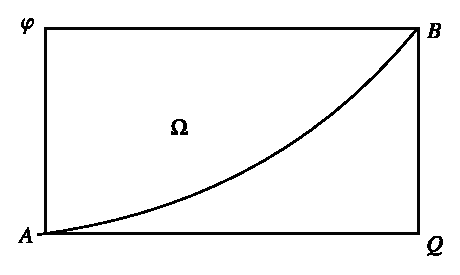
\includegraphics{chap1/6.eps}
\end{figure}
\begin{align*}
\int F \ dx \ dy &= \int \dfrac{\partial u}{\partial x \partial y}dx \ dy\\[3pt]
&= -\frac{1}{2}\int\limits^{P}_{B}\frac{\partial u}{\partial x} dx +\frac{1}{2}\int\limits^{A}_{P}\frac{\partial u}{\partial y}dy + \frac{1}{2}\int\limits^{B}_{A}\left(-\frac{\partial u}{\partial x}dx+\frac{\partial u}{\partial y}dy\right)\\[3pt]
&= \frac{1}{2}(u(B)-u(P)+\frac{1}{2}(u(A)-u(P))+\frac{1}{2}\int\limits^{B}_{A}-\frac{\partial u}{\partial x}dx+\frac{\partial u}{\partial y}dy.
\end{align*}
\footnote[7]{Hence 
$$
u(P)=-\int\limits_{\Omega} F \ dx \ dy +\frac{1}{2}(u(A)+u(B))+\frac{1}{2}\int\limits^{B}_{A}\frac{\partial u}{\partial x}dx-\frac{\partial u}{\partial y}dy
$$}

When $Q$ is below the curve, we have
$$
u(Q)=-\int\limits_{\Omega} F \ dx \ dy +\frac{1}{2}(u(A)+u(B))-\frac{1}{2}\int\limits^{B}_{A}\left(\frac{\partial u}{\partial x}dx-\frac{\partial u}{\partial y}\right)dy
$$

When the initial data are zero on $S$, we have in this case
$$
u(P)=-\int\limits_{\Omega}F \ dx \ dy.
$$

We will not check here that the function $u(P)$ defined by this formula effectively solves the Cauchy problem. This will be done in a more general context later.

\section*{Riemann's Formula:}\pageoriginale

We will now generalise the above representation of the solution of the Cauchy problem to the case $Lu=F$ where $L$ is an hyperbolic operator of the form:
$$
L=\frac{\partial^{2}}{\partial x\partial y}+a(x,y)\frac{\partial}{\partial x}+b(x,y)\frac{\partial}{\partial y}+c(x,y)
$$
where $a$, $b$, $c$ are smooth function (Essentially every hyperbolic operator in two variables is of this form at least locally. See the appendix).

We consider the adjoint operator $L^{\ast}$ given by
$$
L^{\ast}(v)=\frac{\partial^{2}v}{\partial x\partial y}-\frac{\partial}{\partial x}(av)-\frac{\partial}{\partial y}(bv)+cv.
$$
A simple calculation yields the formula
$$
vL(u)-uL^{\ast}(v)=\frac{\partial Q}{\partial x}-\frac{\partial P}{\partial y}
$$
where
\begin{align*}
P &= \frac{1}{2}\left(u\frac{\partial v}{\partial x}-v\frac{\partial u}{\partial x}\right)-b \ u \ v\\[3pt]
Q &= \frac{1}{2}\left(v\frac{\partial u}{\partial y}-u\frac{\partial v}{\partial y}\right)+a \ u \ v,
\end{align*}
so that we have for a bounded open set $\Omega$ with piecewise smooth boundary.
$$
\int\limits_{\Omega}vL(u)-uL^{\ast}(v)=\int\limits_{\partial \Omega}Pdx+Qdy
$$
We now apply this to the domain $\Omega$ in the previous section.
\begin{figure}[H]
\centering
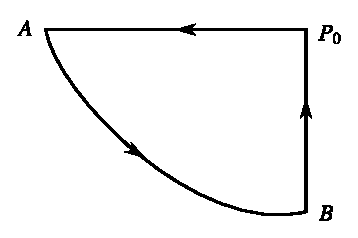
\includegraphics{chap1/7.eps}
\end{figure}

We have
\begin{align*}
\int\limits^{P_{0}}_{B}Pdx+Qdy=\int\limits^{P}_{P_{0}}Qdy &= \int\limits^{P_{0}}_{B}\frac{1}{2}v\frac{\partial u}{\partial y}dy+\int\limits^{P_{0}}_{B}\left(-\frac{1}{2}u\frac{\partial v}{\partial y}+auv\right)\,dy\\[4pt]
&= \frac{1}{2}uv(P_{0})-\frac{1}{2}uv(B)+\int\limits^{P_{0}}_{B}u\left(-\frac{\partial v}{\partial y}+av\right)\,dy.
\end{align*}\pageoriginale
by integrating by parts the first term. Similarly,
\begin{align*}
\int\limits^{A}_{P_{0}}Pdx+Qdy=\int\limits^{A}_{\tau_{0}}Pdx &= -\frac{1}{2}\int\limits^{A}_{P_{0}}v\frac{\partial u}{\partial x}dx+\int\limits^{A}_{P_{0}}\left(\frac{1}{2}u\frac{\partial y}{\partial x}-buv\right)\,dx\\[4pt]
&= -\frac{1}{2}\left\{uv(A)-uv(P_{0})\right\}+\int\limits^{A}_{P_{0}}u\frac{\partial v}{\partial x}-buv \ dx\\[4pt]
&= \frac{1}{2}uv(P_{0})-\frac{1}{2}uv(A)+\int\limits^{A}_{P_{0}}u\left(\frac{\partial v}{\partial x}-bv\right)\,dx
\end{align*}
Suppose that we can choose for each $P_{0}=(x_{0},y_{0})$ a function $R(x,y,x_{0},y_{0})$ such that
\begin{enumerate}
\renewcommand{\labelenumi}{(\theenumi)}
\item $L^{\ast}_{x,y}R=0$.

\item $\dfrac{\partial R}{\partial x}=bR$ \ on the line \ $[P_{0},A]$ \ i.e. on \ $y=y_{0}$ and $\dfrac{\partial R}{\partial y}=R$ on the line $[B, P_{0}]$ i.e., on $x=x_{0}$

\item $R(x_{0},y_{0},x_{0},y_{0})=1$.
\end{enumerate}

Then we find from the above formula, choosing $v=R$,
\begin{align*}
u(P_{0}) &= \frac{1}{2}\left\{Ru(A)+Ru(B)\right\}\\[3pt]
         &\quad + \int\limits^{B}_{A}\left\{\frac{1}{2}R\frac{\partial u}{\partial x}+\left(bR-\frac{1}{2}\frac{\partial R}{\partial x}\right)u\right\}\,dx\\[3pt]
&\quad - \int\limits^{B}_{A}\left\{\frac{1}{2}R\frac{\partial u}{\partial y}+\left(aR-\frac{1}{2}\frac{\partial R}{\partial y}\right)u\right\}\,dy\\[3pt]
&\quad + \int\limits_{\Omega} RF \ dx \ dy.
\end{align*}
Such\pageoriginale a function $R(x,y,x_{0},y_{0})$ depending on $(x_{0},y_{0})$ is called the Riemann function for $L$ with respect to $(x_{0},y_{0})$ and the above formula is called the {\em Riemann's formula}. Note that conditions (2) and (3) give that
$$
R(x,y_{0},x_{0},y_{0})=\exp \int\limits^{x}_{x_{0}}b(x,y_{0})\,dx
$$
and
$$
R(x_{0},y,x_{0},y_{0})=\exp \int\limits^{y}_{y_{0}}Q(x_{0},y)\,dy
$$
\begin{figure}[H]
\centering
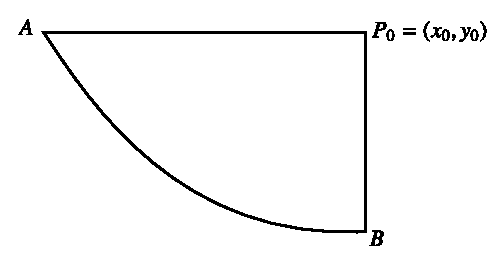
\includegraphics{chap1/8.eps}
\end{figure}
\noindent
Thus to find a Riemann funciton, we have to find a solution $u$ of the adjoint equation such that values of $u$ coincide with a given function on the union of the two characteristics through $P_{0}$. Thus we have a characteristic {\em Cauchy problem}.

\section*{Characteristic Cauchy Problem:}

Regarding the characteristic Cauchy problem, we have

\begin{theorem*}
Let $(0ABC)$ be a rectangle where $0=(0,0)$. Consider the differential operator $\dfrac{\partial^{2}}{\partial x\partial y}-a\dfrac{\partial}{\partial x}-b\dfrac{\partial}{\partial y}-d$ where
\begin{figure}[H]
\centering
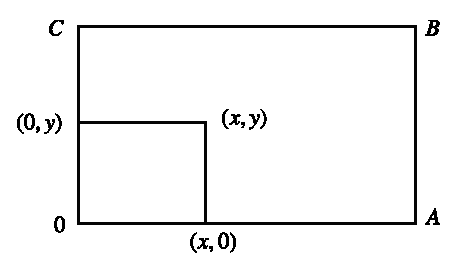
\includegraphics{chap1/9.eps}
\end{figure}
\noindent
$a$, $b$, $c$\pageoriginale are $c^{\infty}$ functions in $\Omega$ where $\Omega$ is the interior of the ractangle. Let $\phi(x)$ (resp. $\psi(y)$) be a $C^{2}$ function in the closed interval $(0,A)$ (resp. interval $0c$) such that $\phi(0)=\psi(0)$ and $F$ a $c^{1}$ function in $\overline{\Omega}$. Then there exists a unique $C^{2}$ function $u$ in $\overline{\Omega}$ such that
\begin{enumerate}
\renewcommand{\labelenumi}{\rm(\theenumi)}
\item $\dfrac{\partial^{2}u}{\partial x\partial y}-a\dfrac{\partial u}{\partial x}-b\dfrac{\partial u}{\partial y}-cu=F$ \ in \ $\Omega$

\item $u(x,0)=\phi(x)$ \ on \ $OA$ \ and \ $u(0,y)=\psi(y)$ \ on \ $0c$.
\end{enumerate}
\end{theorem*}

\section*{Preliminaries. Neumann Series. Volterra Kernel:}\pageoriginale

Before proceeding to the proof of the theorem, let us consider the special case of the operator $\dfrac{\partial^{2}}{\partial x\partial y}$. (This is obtained by looking at the operators $\dfrac{\partial^{2}}{\partial x\partial y}+\lambda\left(-a\dfrac{\partial}{\partial x}-b\dfrac{\partial}{\partial y}-d\right)$ where $\lambda$ is a real parameter. For $\lambda=0$, we have $\dfrac{\partial^{2}}{\partial x\partial y}$ and for $\lambda=1$, we obtain the original operator) If $\dfrac{\partial^{2}u_{0}}{\partial x\partial y}=F$ we have, for $(x,y)\in \Omega$,
$$
\int\limits^{x}_{0}\int\limits^{y}_{0}F(\xi,\eta)d\xi d\eta =\int\limits^{x}_{0}\int\limits^{y}_{0}\dfrac{\partial^{2}u_{0}}{\partial x\partial y}=\int \dfrac{\partial u_{0}}{\partial \eta}
$$
where the line integral is taken over the rectangle with vertices $(0,0)$, $(x,0)$, $(x,y)$ and $(0,y)$. Thus $u_{0}(x,y)=\phi(x)-\phi(0)+\psi(y)+\int\limits^{x}_{0}\int\limits^{y}_{0}F(\xi,\eta)d\xi d\eta$. Now, if we define $u_{0}(x,y)$ by this formula, we check easily that $u_{0}$ is $C^{2}$ in $\overline{\Omega}$ and satisfies conditions (1) and (2) (with $u=u_{0}$, $a=b=d=0$).

Note incidentally that the above formula shows that we cannot prescribe arbitrarily `Dirichlet data' for the operator $\dfrac{\partial^{2}}{\partial x\partial y}$ on all the four sides of the rectangle.

Going over to the general case and writing (1) in the form
$$
\frac{\partial^{2}u}{\partial x \partial y}=\left(a\frac{\partial u}{\partial x}+b\frac{\partial u}{\partial y}+du\right)+F
$$
we must have, by applying the above argument to the function on the right hand side, that
\begin{align*}
u(x,y)=\Big\{ \phi(x) &- \phi(0)+\psi(y)+\int\limits^{x}_{0}\int\limits^{y}_{0}F(\xi,\eta) d\xi d\eta\Big\}+\\[4pt]
& + \int\limits^{x}_{0}\int\limits^{y}_{0}\left(a(\xi,\eta)\frac{\partial u}{\partial \xi}+b\frac{\partial u}{\partial\eta}+du\right)d\xi \ d\eta
\end{align*}
If we call the function in the curly brackets as $u_{0}$ and the last term on the right as $Ku$ we can write this equation in the form
$$
u=u_{0}+Ku,
$$\pageoriginale
where $u_{0}$ is known. We may view $u\to Ku$ as a continuous linear map in a suitable (normed) function space. The relation can be written as
$(I-K)u=u_{0}$ where $I$ is the identity operator. Now, formally,
$$
u=(I-K)^{-1}u_{0}=(I+K+K^{2}+\cdots)u_{0}=u_{0}+Ku_{0}+K^{2}u_{0}+\cdots
$$
where $K^{n}$ denotes the $n^{\text{th}}$ iterate of $K$. If this series (the ``Neumann Series'') converges in the function space for every $u_{0}$, we would have solved the above equation. Moreover, this solution would be unique. For if $u$ and $u'$ are two solutions $\omega=u-u'$ would satisfy $\omega=K\omega$. Since the series $\sum K^{n}\omega$ converges $K^{n}\omega\to 0$ as $n\to \infty$ while $\omega=K^{n}\omega$ for all $n$. This implies that $\omega=0$.

As an example, consider the operator $K$ given by 
$$
Ku(x)=\int\limits^{1}_{0}K(x,y)u(y)dy
$$
where $K(x,y)$ is a function on $(0,1)\times (0,1)$ satisfying $K(x,y)=0$ for $0\leq x\leq y\leq 1$ and continuous in $0\leq y\leq x\leq 1$. (A function $K(x,y)$ of this type is said to be a {\em Volterra Kernel}).
\begin{figure}[H]
\centering
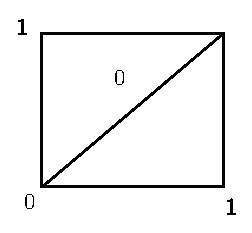
\includegraphics{chap1/10.eps}
\end{figure}
\noindent
Consider $K$ as an operator, say, on the space of bounded measurable functions on $(0,1)$ and let us solve the equation $u=u_{0}+Ku$. We have
$$
Ku_{0}(x)=\int\limits^{x}_{0}K(x,y)u_{0}(y)dy
$$
Let $|K(x,y)|\leq M$ and $|u_{0}(y)|\leq A$ for $x$, $y\in (0,1)$. Then we have
\begin{align*}
|Ku_{0}(x)| &\leq MA \int\limits^{x}_{0}dy=MAx\\[3pt]
|K(Ku_{0}(x))| &= |\int\limits^{x}_{0}K(x,y)(Ku_{0})(y)dy|\\[3pt]
&\leq M^{2}A\int\limits^{x}_{0}y \ dy\\[3pt]
&\leq AM^{2}\frac{x^{2}}{2}.
\end{align*}\pageoriginale
Similarly, we have, by induction, that
$$
|K^{2}u_{0}(x)|\leq AM^{n}\dfrac{x^{n}}{n!}
$$
In particular, we have $|K^{n}u_{0}(x)|\leq \dfrac{AM^{n}}{n!}$. Thus the series
$$
\sum\limits_{n\geq 1} K^{n}u_{0}(x)
$$
is dominated by the exponential series
$$
\sum\limits_{n\geq 1} \dfrac{AM^{n}}{n!}
$$
and hence converges uniformly in $(0,1)$. Thus $u=u_{0}+\sum\limits_{n\geq 1}K^{n}u_{0}$ is in our space and satisfies
$$
u=u_{0}+\int\limits^{1}_{0}K(x,y)u(y)dy.
$$

We will use a similar method to solve the characteristic Cauchy problem.

\section*{Proof of the Theorem on the Characteristic Cauchy Problem:}

Define
$$
u_{0}=\phi(x)-\phi(y)+\psi(y)+\int\limits^{x}_{0}\int\limits^{y}_{0}F(\xi,\eta)d\xi d\eta
$$
and $u_{n}(n\geq 1)$ inductively by
$$
u_{n}(x,y)=\int\limits^{x}_{0}\int\limits^{y}_{0}\left(a\frac{\partial u_{n-1}}{\partial \xi}+b\dfrac{\partial u_{n-1}}{\partial \eta}+du_{n-1}\right)d\xi \ d\eta.
$$\pageoriginale
Note that if $u_{n-1}$ is of class $C^{1}$ (resp. $C^{2}$), so is $u_{n}$ (see below). We shall show that the series $u_{0}+\sum\limits_{n\geq 1}u_{n}$ and the series obtained by taking partial derivatives upto order two of the terms converge uniformly in $\overline{\Omega}$.

Suppose that we have for $(x,y)\in \overline{\Omega}$
\begin{align*}
& |u_{n-1}(x,y)|\leq H\frac{(x+y)^{n}}{n!}\\[3pt]
& \left|\frac{\partial u_{n-1}}{\partial x}(x,y)\right|\leq H\frac{(x+y)^{n-1}}{(n-1)!}\tag{*}\\[3pt]
& \left| \frac{\partial u_{n-1}}{\partial y}(x,y)\right|\leq H \frac{(x+y)^{n-1}}{n-1!}
\end{align*}
with some positive constant $H$. Let $M$ be a positive number such that $|a(x,y)|\leq M$, $|b(x,y)|\leq M$ and $|d(x,y)|\leq M$ for $(x,y)\in \overline{\Omega}$. We then have
$$
|u_{n}(x,y)|\leq \int\limits^{x}_{0}\int\limits^{y}_{0}MH\left[2\frac{(\xi+\eta)^{n-1}}{(n-1)!}+\frac{(\xi+\eta)^{n}}{n!}\right]d\xi \ d\eta
$$
Now
\begin{align*}
\int\limits^{x}_{0}\int\limits^{y}_{0}\frac{(\xi+\eta)^{n}}{n!}d\xi \ d\eta &= \int\limits^{x}_{0}\left\{\frac{(\xi+y)^{n+1}}{(n+1)!}-\frac{\xi^{n+1}}{(n+1)!}\right\}\,d\xi\\[3pt]
&= \frac{(x+y)^{n+2}}{(n+2)!}-\frac{y^{n+2}}{(n+2)!}-\frac{x^{n+2}}{(n+2)!}\\[3pt]
&\leq \frac{(x+y)^{n+2}}{(n+2)!}
\end{align*}
Estimating\pageoriginale similarly the other term under the integral sign, we find that
$$
|u_{n}(x,y)|\leq H\frac{(x+y)^{n+1}}{(n+1)!}\left[2M+M\frac{(x+y)}{n+2}\right]
$$
Now
\begin{align*}
\left|\frac{\partial u_{n}}{\partial x}(x,y)\right| &= \left|\int\limits^{y}_{0}a(x,\eta)\frac{\partial u_{n}}{\partial x}(x,\eta)+b(x,n)\frac{\partial u_{n}}{\partial \eta}(x,\eta)+c(x,\eta)u_{n}d\eta\right|\\[3pt]
&\leq H\int\limits^{y}_{0}\left[2M\frac{(x+\eta)^{n-1}}{n-1!}+M\frac{(x+\eta)^{n}}{n!}\right]d\eta\\[3pt]
&\leq 2HM \frac{(x+y)^{n}}{n!}+HM\frac{(x+y)^{n+1}}{(n+1)!}\\[3pt]
&\leq H\frac{(x+y)^{n}}{n!}\left[2M+M\frac{(x+y)}{(n+1)}\right]
\end{align*}
and we have the same estimate for $\dfrac{\partial u_{n}}{\partial y}$. Now if $K$ is a positive constant such that $K\geq 2M+M(x+y)$ for all $(x,y)$ in $\overline{\Omega}$ we have
\begin{align*}
& |u_{n}(x,y)|\leq HK \frac{(x+y)^{n+1}}{(n+1)!}\\[3pt]
& \left| \frac{\partial u_{n}}{\partial x}(x,y)\right| \leq HK \frac{(x+y)^{n}}{n!}\\[3pt]
& \left|\frac{\partial u_{n}}{\partial y}(x,y)\right| \leq HK \frac{(x+y)^{n}}{n!} 
\end{align*}
Thus we have an estimate for $u_{n}$ similar to that of $u_{n-1}$ except that the constant $H$ is replaced by $H$, $K$, where $K$ depends only on $M$ and the size of the rectangle.

Let $L$ be a positive number such that
$$
|u_{0}(x,y)|\;\left|\frac{\partial u_{0}}{\partial x}(x,y)\right|\quad\text{and}\quad \left|\frac{\partial u_{0}}{\partial y}(x,y)\right|
$$
are all less than or equal to $L$ for $(x,y)$ in $\overline{\Omega}$. We then have
\begin{align*}
& |u_{1}(x,y)| \leq 3ML \int\limits^{x}_{0}\int\limits^{y}_{0}dx \ dy = 3ML \ xy \leq 3ML \frac{(x+y)^{2}}{2}\\[3pt]
& \left|\frac{\partial u_{1}}{\partial x}(x,y)\right| \leq 3ML \int\limits^{y}_{0}dy = 3MLy\leq 3ML (x+y)
\end{align*}\pageoriginale
and similarly for $\dfrac{\partial u_{1}}{\partial y}(x,y)$. By induction, we conclude that, for $n\geq 1$,
\begin{align*}
& |u_{n}(x,y)| \leq 3ML \ K^{n-1}\frac{(x+y)^{n+1}}{(n+1)!}\\[3pt]
& \left|\frac{\partial u_{n}}{\partial x}(x,y)\right|\leq 3ML \ K^{n-1}\frac{(x+y)^{n}}{n!}
\end{align*}
and
$$
\left|\frac{\partial u_{n}}{\partial y}(x,y)\right|\leq 3ML \ K^{n-1}\frac{(x+y)^{n}}{n!}
$$
Thus the series $\sum\limits^{\infty}_{n=0}u_{n}(x,y)$ converges uniformly, say to $u$, along with the series of first partial derivatives. If $S_{n}=\sum\limits^{n}_{k=0}u_{k}$, we have
$$
S_{n}=u_{0}+\int\limits^{x}_{0}\int\limits^{y}_{0}\left(a\frac{\partial S_{n-1}}{\partial \xi}+b\frac{\partial S_{n-1}}{\partial \eta}+dS_{n-1}\right)d\xi \ d\eta.
$$
Using uniform convergence of the sequence $S_{n}$ and the sequence of first partial derivatives, we get in the limits a $C^{1}$ function $u$ satisfying
$$
u=u_{0}+\int\limits^{x}_{0}\int\limits^{y}_{0}\left(a\frac{\partial u}{\partial \xi}+b\frac{\partial u}{\partial \eta}+du\right)d\xi \ d\eta.
$$
Let us prove that $u$ is of class $C^{2}$. Note that since $u_{0}$ is $C^{2}$, all the $u_{n}$ are $C^{2}$. Assume, in addition to (*), that
$$
\left| D^{\alpha}u_{n-1}\right|\leq H \frac{(x+y)^{n-2}}{(n-2)!}\quad\text{for}\quad |\alpha|=2
$$
Then
\begin{align*}
& \frac{\partial u_{n}}{\partial x}=\int\limits^{y}_{0}a(x,\eta)\frac{\partial u_{n-1}}{\partial x}+b(x,\eta)\frac{\partial u_{n-1}}{\partial \eta}+d(x,\eta)u_{n-1}(x,\eta)d\eta\\[3pt]
& \frac{\partial^{2}u_{n}}{\partial x}=\int\limits^{y}_{0}\left\{\frac{\partial a}{\partial x}\frac{\partial u_{n-1}}{\partial x}+a\frac{\partial^{2}u_{n-1}}{\partial x^{2}}+\frac{\partial b}{\partial x}\frac{\partial u_{n-1}}{\partial \eta}+b\frac{\partial^{2}u_{n-1}}{\partial x^{2}}+\right.\\[3pt]
&\qquad\qquad \left. + u_{n-1}\frac{\partial d}{\partial x}+\frac{\partial u_{n-1}}{\partial x}d\right\}\,d\eta
\end{align*}\pageoriginale
Let $M$ be an upper bound for $a$, $b$, $d$ and their first partial derivatives in the domain. As before, the first, third and the last terms are each majorised in modulus by $HM\dfrac{(x+y)^{n}}{n!}$ and the fifth term by $HM\dfrac{(x+y)^{n+1}}{n+1!}$. Now,
$$
\left| \int\limits^{y}_{0}a\frac{\partial^{2}u_{n-1}}{\partial x^{2}}d\eta \right|\leq \int\limits^{y}_{0}MH\frac{(x+y)^{n-2}}{n-2!}dy\leq MH \frac{(x+y)^{n-1}}{(n-1)!}
$$
and we have the same estimate for the fifth term. Thus
\begin{align*}
\left| \frac{\partial^{2}u_{n}}{\partial x^{2}}\right| &\leq H\frac{(x+y)^{n-1}}{(n-1)!}\left(2M+3M \frac{(x+y)}{n}+\frac{M(x+y)^{2}}{n(n+1)}\right)\\[3pt]
&\leq H\frac{(x+y)^{n-1}}{n-1!}\left(2M+3M(x+y)+M(x+y)^{2}\right)\\[3pt]
&\leq HK \frac{(x+y)^{n-1}}{n-1!}
\end{align*}
if we choose for $K$ a positive number such that
$$
K\geq 2M + 3 (M\in x+y)+M(x+y)^{2}
$$
for all $(x,y)$ in the rectangle. Similarly
$$
|D^{\alpha}u_{n}|\leq HK\frac{(x+y)^{n-1}}{n-1!}\quad\text{for}\quad |\alpha|=2.
$$
\begin{align*}
\left| \frac{\partial^{2}u_{n}}{\partial x\partial y}\right| &= \left| a\frac{\partial u_{n-1}}{\partial x}+b\frac{\partial u_{n-1}}{\partial y}+du_{n-1}\right|\\[3pt]
&\leq H\frac{(x+y)^{n-1}}{n-1!}(2M+x+y)\\[3pt]
&\leq KH \frac{(x+y)^{n-1}}{n-1!}
\end{align*}
We\pageoriginale also have
$$
\left| \frac{\partial^{2}u_{n}}{\partial y^{2}}\right|\leq KH \frac{(x+y)^{n-1}}{n-1!}.
$$

If we choose $H$ such that $H\geq 3ML$ and $H\geq |D^{\alpha}u_{1}(x,y)|$, for $|\alpha|=2$, $(x,y)$ rectangle, we see that we can start the induction.

Thus the series of second partial derivatives of $\sum u_{n}$ also converge uniformly. Hence $u$ is $C^{2}$.

It is easy to check, using
$$
u=u_{0}+\int\limits^{x}_{0}\int\limits^{y}_{0}\left(a\frac{\partial u}{\partial \xi}+b\frac{\partial u}{\partial \eta}+du\right)d\xi \ d\eta,
$$
that $u$ is a solution of the characteristic Cauchy problem.

To prove the uniqueness let $u$ and $V$ be two solutions of the problem. Then $\omega=u-v$ satisfies
\begin{align*}
\omega &= \int\limits^{x}_{0}\int\limits^{y}_{0}\left(a\frac{\partial \omega}{\partial \xi}+b\frac{\partial \omega}{\partial \eta}+du\right)d\xi \ d\eta\\[4pt]
&= S\omega,\qquad\text{say}
\end{align*}
By our estimates, $S^{n}\omega$ converges uniformly to zero. Hence $\omega=0$.

This completes the proof of the theorem.

\section*{Riemann's Method for Solving the Cauchy Problem:}

As before, we are given a curve $S$, $y=\sigma (x)$, with, say, $\sigma \ a \ C^{2}$ functions of $x$ with $\sigma'(x)<0$. We are also given $C^{2}$ functions $\phi_{0}$, $\phi_{1}$ on $S$ which may viewed as $C^{2}$ functions $\phi_{0}$, $\phi_{1}$ of $x$. Let $M$, $N$ be two points on $S$. Let $\Omega$ be the rectangular region formed by the parallels to the\pageoriginale $x$, $y$ axes through $M$ and $N$.
\begin{figure}[H]
\centering
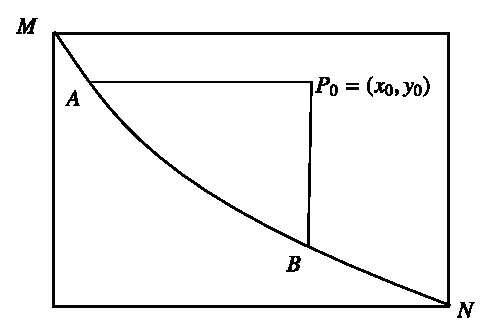
\includegraphics{chap1/11.eps}
\end{figure}
\noindent
Assume that coefficients $a$, $b$, $d$ of the operator are $C^{\infty}$ on $\overline{\Omega}$. Let $F$ be a $C^{1}$ function on $\overline{\Omega}$. We have to find a function $u$ in $\Omega$ such that $Lu=F$, $u\big|_{S}=\phi_{0}$ and, say $\left.\dfrac{\partial u}{\partial y}\right|_{S}=\phi_{1}$ (the value of $\dfrac{\partial u}{\partial x}$ on $S$ is also known is given by
$$
\left(\dfrac{\partial u}{\partial x}\right)_{y=\sigma(x)}-\phi'_{0}(x)=\phi_{1}(x)\sigma'(x)).
$$

We may reduce the problem to one where the initial data are zero by changing $F$. In fact, if $\omega=u-\phi_{0}(x)-[y-\sigma(x)]\phi_{1}(x)$, then $L\omega=F+G$, where $G$ is a $C^{1}$ function and $\omega$ has zero Cauchy data on $S$. So,, if we find $\omega$, we know $u$. From now on we assume that the Cauchy data are zero.

Let us concentrate on the region above the curve in $\Omega$. Similar consideration will apply for the region below.

In our present case, where the initial data are zero, Remann's formula reduces to
$$
u(x_{0},y_{0})=\int\limits_{\Omega(x_{0},y_{0})}R(\xi, \eta, x_{0},y_{0})d\xi \ d\eta
$$
where $R(\xi,\eta,x_{0})$ is the Riemann function for $L$ with respect $(x_{0},y_{0})$ and $(x_{0},y_{0})$ is the region formed by the characteristics through $P_{0}=(x_{0},y_{0})$\pageoriginale and $S$. Now we $k$ can find the Riemann funciton by solving a characteristic Cauchy problem and we may then define $u(x_{0},y_{0})$ by the above formula. But then, it is not even clear that for fixed $(\xi,\eta)$, $R(\xi,\eta,x_{0},y_{0})$ is a $C^{2}$ function of $(x_{0},y_{0})$ in the shaded region. To see this and for 
\begin{figure}[H]
\centering
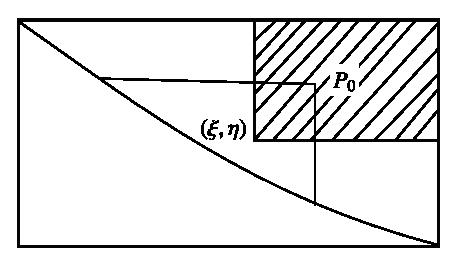
\includegraphics{chap1/12.eps}
\end{figure}
proving that the above formula solves the Cauchy problem, we need

\section*{Reciprocity Law for the Riemann Function:}

\begin{prop*}
Let $P$ and $D$ be two distincts points in $\mathbb{R}^{2}$. Let $[D \ B \ P \ A]$ be the closed rectangular formed by parallels to $x$ and $y$ axis through $D$ and $P$. Suppose that the coefficients of $L$ are $C^{\infty}$ in a neighbourhood of $[D \ B \ P \ A]$.
\begin{figure}[H]
\centering
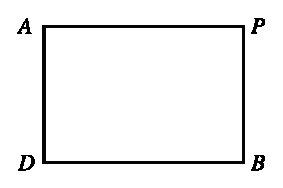
\includegraphics{chap1/13.eps}
\end{figure}
\end{prop*}

Let $R_{P}$ (resp. $R^{*}_{D}$) denote the Riemann function for $L$ (resp. the adjoint operator $L^{*}$) with respect to $P$ (resp. $D$) (Note that $R_{P}$ and $R^{*}_{D}$ are defined in $[D \ B \ P \ A]$). We then have
$$
R_{P}(D)=R^{*}_{D}(P).
$$

\begin{remark*}
This\pageoriginale may be interpreted as follows. If $R(\xi, \eta, x_{0}, y_{0})$ is the Riemann function for $L$ with respect $(x_{0},y_{0})$ and if $(x_{0},y_{0})$ are considered as variables with $(\xi,\eta)$ fixed, then $R$ becomes the Riemann function for the adjoint operator $L^{*}$ with respect to $(\xi,\eta)$. Since $(L^{*})^{-}=L$, considered as function of $(x_{0},y_{0})$, $R$ is a solution of the original operator $L$.
\end{remark*}

\section*{Proof of the Proposition:}

Let $u$ be a $C$ function in $[D \ B \ P \ A]$ satisfying $Lu=0$. We apply the Riemann formula for $[D \ B \ P \ A]$. (In the earlier proof of this formula we replace the arc $AB$ by the broken arc $A$ $D$ $B$). We then have, with $R=R_{P}$,
\begin{align*}
u(P) &= \frac{1}{2}\{u(A)R(A)+u(B)R(B)\}\\[3pt]
&+\frac{1}{2}\int\limits^{B}_{D}\left(R\frac{\partial u}{\partial x}-\frac{\partial R}{\partial x}u+2b \ Ru\right)dx\\[4pt]
&-\frac{1}{2}\int\limits^{D}_{A}\left(R\frac{\partial u}{\partial y}-\frac{\partial R}{\partial y}u+2A \ Ru\right)dy
\end{align*}
The second term on the right is equal to
\begin{align*}
 &\frac{1}{2}\int\limits^{B}_{D}\left[-\frac{\partial}{\partial x}(Ru)+2R\frac{\partial u}{\partial x}+2b \ Ru\right]dx\\[3pt]
= & \frac{1}{2} Ru (D)-\frac{1}{2} Ru (B)+\int\limits^{B}_{D}R\left(\frac{\partial u}{\partial x}+bu\right)dx
\end{align*}
while the last term is equal to
\begin{align*}
& -\frac{1}{2}\int\limits^{D}_{A}\left[-\frac{\partial}{\partial y}(Ru)+2R\frac{\partial u}{\partial y}+2a \ Ru\right]dy\\[3pt]
&= \frac{1}{2} Ru (D)-\frac{1}{2} Ru (A) -\int\limits^{D}_{A}2R\left(\frac{\partial u}{\partial y}+au\right)dy
\end{align*}
We choose $u$ to be the Riemann function for $L^{*}$ with respect to $D$.

We\pageoriginale have $Lu=(L^{*})^{*}u=0$. Note that
$$
L^{*}=\dfrac{\partial^{2}}{\partial x\partial y}-a\frac{\partial}{\partial x}-b\frac{\partial}{\partial y}-d
$$
where $d=\dfrac{\partial a}{\partial x}+\dfrac{\partial b}{\partial y}-C$. Hence $\dfrac{\partial u}{\partial x}+bu=0$ on $DB$ and $\dfrac{\partial u}{\partial y}+au=0$ on $AD$ by the definition of the Riemann function for $L^{*}$ with respect to $D$; moreover $u(D)=1$. Hence we obtain
$$
R^{*}_{D}(P)=R_{P}(D).
$$

\section*{Solution of the Cauchy Problem:}

We shall show in this section that the function
$$
u(x_{0},y_{0})=\iint\limits_{\Omega(x_{0},y_{0})}R(\xi,\eta,x_{0},y_{0})F(\xi,\eta)d\xi \ d\eta
$$
\begin{figure}[H]
\centering
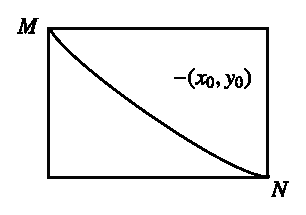
\includegraphics{chap1/14.eps}
\end{figure}
\noindent
is a $C^{2}$ function (in the rectangular region shown in the figure) having zero initial data on $S$ and satisfies $Lu=F$.

We shall consider $(x_{0},y_{0})$ lying above $S$. It is clear that $u$ is continuous upto $S$ and is zero on $S$ as $\Omega(x_{0},y_{0})$ shrinks to a point as we approach $S$. To see the behaviour of the first derivatives on $S$, we use

\begin{lemma*}
We have
\begin{align*}
\frac{\partial u}{\partial x_{0}} &= \int\limits^{P_{0}}_{B}R(x_{0},\eta,x_{0},y_{0})F(x_{0},\eta)dn\\[3pt]
&\quad + \int\limits_{\Omega(x_{0},y_{0})}\dfrac{\partial R}{\partial x_{0}}(\xi, \eta, x_{0}, y_{0})F(\xi, \eta)d\xi \ d\eta
\end{align*}
and\pageoriginale
\begin{align*}
\frac{\partial u}{\partial y_{0}} &= \int\limits^{P_{0}}_{A}R(\xi,y_{0},x_{0},y_{0})F(\xi,y_{0})d\xi\\[3pt]
&\quad + \int\limits_{\Omega(x_{0},y_{0})}\frac{\partial R}{\partial y_{0}}(\xi, \eta, x_{0},y_{0})F(\xi,\eta)d\xi \ d\eta
\end{align*}
\begin{figure}[H]
\centering
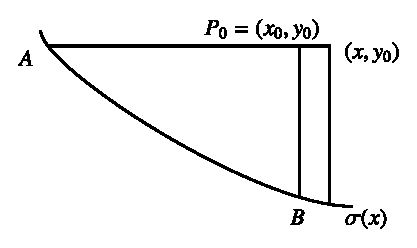
\includegraphics{chap1/15.eps}
\end{figure}
\end{lemma*}

\begin{proof}
We use the following well=known formula (See e.g. Goursat Vol. I, Ch. IV, (98). If
$$
\psi(t)=\int\limits^{b(t)}_{a(t)}h(s,t)ds
$$
then
$$
\frac{d\psi}{dt}=\int\limits^{b(t)}_{a(t)}\frac{\partial h}{\partial t}(s,t)ds+\dfrac{db}{dt}h(b(t),t)-\dfrac{da}{dt}h(a(t),t)
$$
Apply this to the function
\begin{align*}
\psi(x) &= \int\limits_{\Omega(x_{0},y_{0})}R(\xi,\eta,x,y_{0})F(\xi,\eta)d\xi \ d\eta\\[3pt]
&= \int\limits^{(x,y_{0})}_{A}d\xi \left\{\int\limits^{y_{0}}_{\sigma(x)}R(\xi,\eta,x,y_{0})d\eta\right\}\\[3pt]
&= \int\limits^{(x,y_{0})}_{A}h(\xi,x)d\xi
\end{align*}
where $h(x,\xi)$ is the function under the curly bracket. We get
\begin{align*}
\frac{\partial u}{\partial x_{0}}=\left(\frac{d\psi}{dx}\right)_{x=x_{0}} &= \int\limits^{(x_{0},y_{0})}_{A}\frac{dh(\xi,x)}{dx}d\xi+h(x_{0},x_{0})\\[3pt]
&= \int\limits_{\Omega(x_{0},y_{0})}\frac{\partial R}{\partial x}(\xi, \eta, x_{0}, y_{0})d\xi \ d\eta\\[3pt]
&\quad +\int\limits^{P_{0}}_{B}R(x_{0},\eta,x_{0},y_{0})d\eta
\end{align*}
The\pageoriginale second formula is proved similarly.
\end{proof}

\begin{remark*}
The above formula is essentially a special case of the following more general result. Let $\Omega$ be an oriented smooth $n$ - dimensional maniforl. Let $\omega(t)$ be a family of smooth $n$ - forms on $\Omega$ depending smoothly on a parameter. Let further $\Omega(t)$ be a family of relatively compact subdomains (of $\Omega$), with smooth boundaries, depending smoothly on $t$. We then have
$$
\frac{d}{dt}\int\limits_{\Omega(t)}\omega(t)=\int\limits_{\Omega(t)}\frac{d\omega(t)}{dt}+\int\limits_{\partial \Omega(t)}i_{X(t)}\omega(t)\big|_{\partial \Omega(t)}.
$$
where $X(t)$ is the normal field on $\partial\Omega(t)$ corresponding to the infinitesimal variation (deformation) of the boundary $\partial \Omega(t)$ and $i_{X(t)}$ denotes the interior product with respect to $X(t)$. The normal field is defined only as a section of the normal bundle of $\partial \Omega(t)$ in $\Omega(t)$ but $i_{X(t)}\omega(t)\big|_{\partial \Omega(t)}$ is well-defined (i.e., does not depend on the lift of $X(t)$ in the tangent space of $\Omega$).
\end{remark*}

We now proceed to compute $Lu$. We have
\begin{align*}
\frac{\partial^{2}u}{\partial x_{0}\partial y_{0}} &= \frac{\partial}{\partial y_{0}}\left(\int\limits^{P_{0}}_{B}R(x_{0},\eta,x_{0},y_{0})F(x_{0},\eta\right)d\eta\\[3pt]
&\quad \int\limits_{\Omega(x_{0},y_{0})}\frac{\partial R}{\partial x_{0}}(\xi, \eta, x_{0}, y_{0})F(\xi,\eta)d\xi \ d\eta)\\[3pt]
&= \int\limits^{P_{0}}_{B}\frac{\partial R}{\partial y_{0}}(x_{0},\eta x_{0},y_{0}), \ F(x_{0},\eta)d\eta\\[3pt]
&\quad +R(x_{0},y_{0},x_{0},y_{0})F(x_{0},y_{0})\\[3pt]
&\quad \int\limits_{\Omega(x_{0},y_{0})}\frac{\partial^{2}R}{\partial x_{0}\partial y_{0}}(\xi, \eta, x_{0}, y_{0})F(\xi,\eta)d\xi \ d\eta\\[3pt]
&\quad \int\limits^{P_{0}}_{A}\frac{\partial R}{\partial x_{0}}(\xi, y_{0}, x_{0}, y_{0})F(\xi, y_{0})d\xi
\end{align*}\pageoriginale
Applying the Lemma with $R$ replaced by $\dfrac{\partial R}{\partial x_{0}}$. Hence
\begin{align*}
& \frac{\partial^{2}u}{\partial x_{0}\partial y_{0}}+a(x_{0},y_{0})\frac{\partial u}{\partial x_{0}}+b\frac{\partial u}{\partial y_{0}}+Cu\\[3pt]
&\quad = R(x_{0},y_{0},x_{0},y_{0})F(x_{0},y_{0})\\[3pt]
&\quad +\int\limits^{P_{0}}_{B}\frac{\partial R}{\partial y_{0}}+aR)F(x_{0},\eta)d\eta+\int\limits^{P_{0}}_{A}\left(\frac{\partial R}{\partial x_{0}}+bR\right)F(\xi,y_{0})d\xi\\[3pt]
&\quad +\int\limits_{\Omega (x_{0},y_{0})}\left(\frac{\partial^{2}R}{\partial x_{0}\partial y_{0}}+a(x_{0},y_{0}\right)\frac{\partial R}{\partial x_{0}}+b\frac{\partial R}{\partial y_{0}}+c(x_{0},y_{0})F(\xi,\eta)d\xi \ d\eta =0\\[3pt]
&\quad = F(x_{0},y_{0})
\end{align*}
as $R$ considered as a function of $(x_{0},y_{0})$ is a Riemann funciton for $L^{*}$ so that $R(x_{0},y_{0},x_{0},y_{0})=1\dfrac{\partial R}{\partial y_{0}}+aR=0$ on $BP_{0}$, $\dfrac{\partial R}{\partial x_{0}}+bR=0$ on $AP_{0}$ and $L_{x_{0},y_{0}}R=0$.

Similar calculation would show that $u$ is of class $C^{2}$ upto $S$ (Recall that $(x_{0},y_{0})$ has been taken to be above the curve). Similarly by taking $(x_{0},y_{0})$ below the curve, we have a solution below $S$ which is of class $C^{2}$ upto $S$. To see that $u$ is of class $C^{2}$ in the whole rectangular region we use the following fact if $u$ is a function of class $C^{1}$ in the region and is, on each of the closed half spaces defined by a non-characteristic curve, a $C^{2}$ solution, then $u$ must be of class $C^{2}$ in the region. We have proved 

\begin{theorem*}
Consider in an open set $\Omega$ in $\mathbb{R}^{2}$ the hyperbolic differential operator
$$
L=\frac{\partial^{2}}{\partial x\partial y}+a\frac{\partial}{\partial x}+b\frac{\partial}{\partial y}+c
$$\pageoriginale
where $a$, $b$, $c$ are smooth functions in $\Omega$. Let $S$ be a smooth curve in $\Omega$ given by $y=\sigma(x)$, $\sigma'(x)\neq 0$. Suppose that $M$ and $N$ are two points on $S$ such that the rectangular region $R$ formed by the horizontal and vertical lines through $M$ and $N$ lies completely in $\Omega$. Then there exists a unique $C^{2}$ function $u$ in $R$ such that $Lu=F$ (where $F$ is a given $C^{1}$ function on $\Omega$) and such that $u$ assumes given initial $C^{2}$ Cauchy data on $S$.
\end{theorem*}
